\documentclass[11pt,letterpaper]{article}
\usepackage[utf8]{inputenc}
\usepackage{amsmath,amssymb,fullpage,graphicx}
\usepackage{subfigure}
\let\hat\widehat
\let\tilde\widetilde

\begin{document}
\subsection*{Q1-b}
\begin{verbatim}
n <- 1
sigma <- 1
tau0 <- 1
delta <- seq(-5, 5, by=0.01)
alpha <- 1 - pnorm(sigma * delta / (sqrt(n) * tau0^2))

plot(x=delta, y=alpha, type='l', lwd=3, xlab=expression(delta), ylab=expression(alpha),
     main='Test Size vs delta')
abline(h=c(0, 1), lty=3)
\end{verbatim}

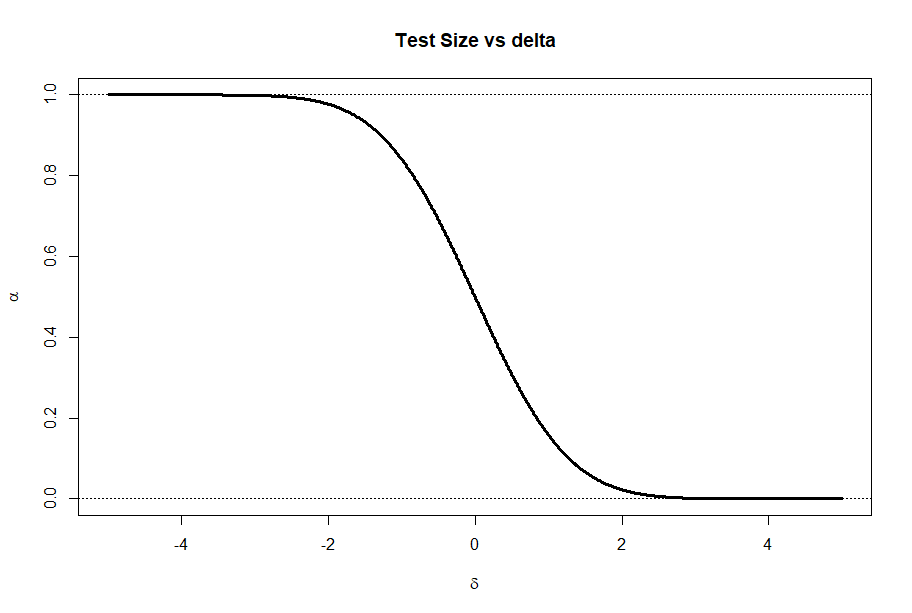
\includegraphics[width=150mm]{q1-b.png}

\noindent From the plot of $\alpha$ versus $\delta = (\theta^{\star} - \theta_0)$, we perceive that the test size decreases as increment of $delta$. The test size or type one error converges to 0 when $\theta_0$, the mean value of $\theta$, is far less than value of $\theta^{\star}$. And the type one error converges to 1 when $\theta_0$ is much bigger than $\theta^{\star}$.

\end{document}